% !TEX program = pdflatex
% !TEX encoding = UTF-8
% !TEX spellcheck = en_US
\documentclass[12pt]{article}

\usepackage[margin=1in]{geometry}
\usepackage[utf8]{inputenc}
\usepackage{amsmath,amsthm,amssymb}
\usepackage{graphicx}
\usepackage{hyperref} % Uso de links
\usepackage[version=4]{mhchem}
\usepackage{siunitx}
\usepackage{enumerate}
\usepackage{titlesec}
\usepackage{booktabs}
\usepackage{bm}
\usepackage{xcolor}

\titleformat{\subsection}
  {\normalfont\large\bfseries}{}{0em}{}

\setlength{\parindent}{0em}

\DeclareMathOperator{\tr}{tr}

\begin{document}

% --------------------------------------------------------------
%                         Start here
% --------------------------------------------------------------

\title{Mechanical Properties of Materials (MSAE 4215), Spring 2019\\ Homework 3 Solutions}
\author{Qi Zhang}
\date{\today}

\maketitle

\tableofcontents
\listoffigures
\listoftables

\section{Problems}
{\color{red} \textbf{Update}:
\begin{itemize}
	\item Remove \textit{parallel axis theorem} in question 2 because it is not required.
	\item Update solution to question 3.
\end{itemize}}

\subsection{4.1}
To monitor strain, it is possible to use optical marks (fiducials) and keep track of them in a
microscope during an experiment. Imagine that there are two fiducials $A$, $B$, separated in $x$ and $y$
by \SI{1}{\centi\meter}. On heating a plate from \SIrange{300}{400}{\kelvin}, fiducial $A$ moves in $(x, y)$ by $(10, 20)$ in
\si{\micro\meter};
fiducial $B$ moves by $(15, 40)$ in \si{\micro\meter}. Assuming that the strain is uniform in the plate, calculate
\begin{itemize}
	\item Drift (total displacement) of the plate

	      \textbf{Solution:}

	      Since $\SI{1}{\micro\meter} = \SI{1e-4}{\centi\meter}$,
	      the distance between $A$ and $B$ is
	      \begin{equation}
		      \overline{AB} = \sqrt{1^2 + 1^2}\,\si{\centi\meter} = \sqrt{2}\,\si{\centi\meter}.
	      \end{equation}
	      The distance between $A'$ and $B'$ is
	      \begin{multline}
		      \overline{A' B'} = \sqrt{(1 + (15 - 10) \times 10^{-4})^2 + (1 + (40 - 20) \times 10^{-4})^2}\,\si{\centi\meter}\\
		      = \sqrt{(1 + 5 \times 10^{-4})^2 + (1 + 2 \times 10^{-3})^2}\,\si{\centi\meter}.
	      \end{multline}
	      The drift is
	      \begin{equation}
		      \overline{A' B'} - \overline{AB} \approx \SI{0.001768}{\centi\meter}.
	      \end{equation}

	\item Rotation of the plate

	      \textbf{Solution:}

	      \begin{align}
		      e_{11} & = \frac{ \partial u_1 }{ \partial x_1 } = \frac{(15 - 10) \times 10^{-4}}{1} = \num{5e-4}, \\
		      e_{12} & = \frac{ \partial u_1 }{ \partial x_2 } = \frac{(15 - 10) \times 10^{-4}}{1} = \num{5e-4}, \\
		      e_{21} & = \frac{ \partial u_2 }{ \partial x_1 } = \frac{(40 - 20) \times 10^{-4}}{1} = \num{2e-3}, \\
		      e_{22} & = \frac{ \partial u_2 }{ \partial x_2 } = \frac{(40 - 20) \times 10^{-4}}{1} = \num{2e-3}.
	      \end{align}
	      Because $[e]$ is neither symmetric nor anti-symmetric, it is a composition of strain and rotation.
	      The rotational portion is
	      \begin{equation}
		      [w] = \begin{bmatrix}
			      0                             & \frac{1}{2} (e_{12} - e_{21}) \\
			      \frac{1}{2} (e_{21} - e_{12}) & 0
		      \end{bmatrix}
		      = \begin{bmatrix}
			      0            & \num{-7.5e-4} \\
			      \num{7.5e-4} & 0
		      \end{bmatrix}.
	      \end{equation}
	      So $\phi = \num{7.5e-4}$.

	\item The tensor strain

	      \textbf{Solution:}

	      It is the symmetric part of $[e]$,
	      \begin{equation}
		      [\varepsilon] = \begin{bmatrix}
			      e_{11}                        & \frac{1}{2} (e_{12} + e_{21}) \\
			      \frac{1}{2} (e_{21} + e_{12}) & e_{22}
		      \end{bmatrix}
		      = \begin{bmatrix}
			      \num{5e-4}    & \num{1.25e-3} \\
			      \num{1.25e-3} & \num{2e-3}
		      \end{bmatrix}.
	      \end{equation}
	\item The thermal expansion coefficient $\alpha$, neglecting any strain normal to the surface.

	      \textbf{Solution:}
	      \begin{equation}
		      \alpha \Delta T = \Delta = \varepsilon_1 + \varepsilon_2 = \tr([\varepsilon]) = \num{2.5e-3},
	      \end{equation}
	      so the thermal expansion coefficient
	      \begin{equation}
		      \alpha = \frac{ \Delta }{ \Delta T } = \frac{ \num{2.5e-3} }{ \SI{400}{\kelvin} - \SI{300}{\kelvin} } = \SI{2.5e-5}{\per\kelvin}.
	      \end{equation}
\end{itemize}

\subsection{2}
Calculate the area moments of inertia relevant for bending, $I_y$, $I_z$, for an
``I"-beam, length $L$ in $x$, cross section in the $yz$ plane formed by:
\begin{itemize}
	\item two horizontal sections, one centered at $y=0$, one centered at $y=W$, width $W$ in $z$, thickness $t$ in $y$,
	\item one vertical section, centered at $z=0$, height $W$ in $y$, thickness $t$ in $z$,
\end{itemize}
joined together to form the shape like a capital ``I".

\textbf{Solution:}

Note there are overlaps between the vertical section and horizontal sections, I will not consider them
for simplicity. It is easy to arrive at a different answer if you choose a different setting of your axes
or integration upper/lower bounds, so do not be shocked if my answer is too dissimilar from yours.

Assume ``centered at $y=0$" means ``centered at $(0, 0, 0)$", ``centered at $y=W$" means
``centered at $(0, W, 0)$", and ``centered at $z=0$" means ``centered at $(0, \frac{W}{2}, 0)$".
See \ref{fig:i-beam} for reference.
\begin{figure}[h]
	\centering
	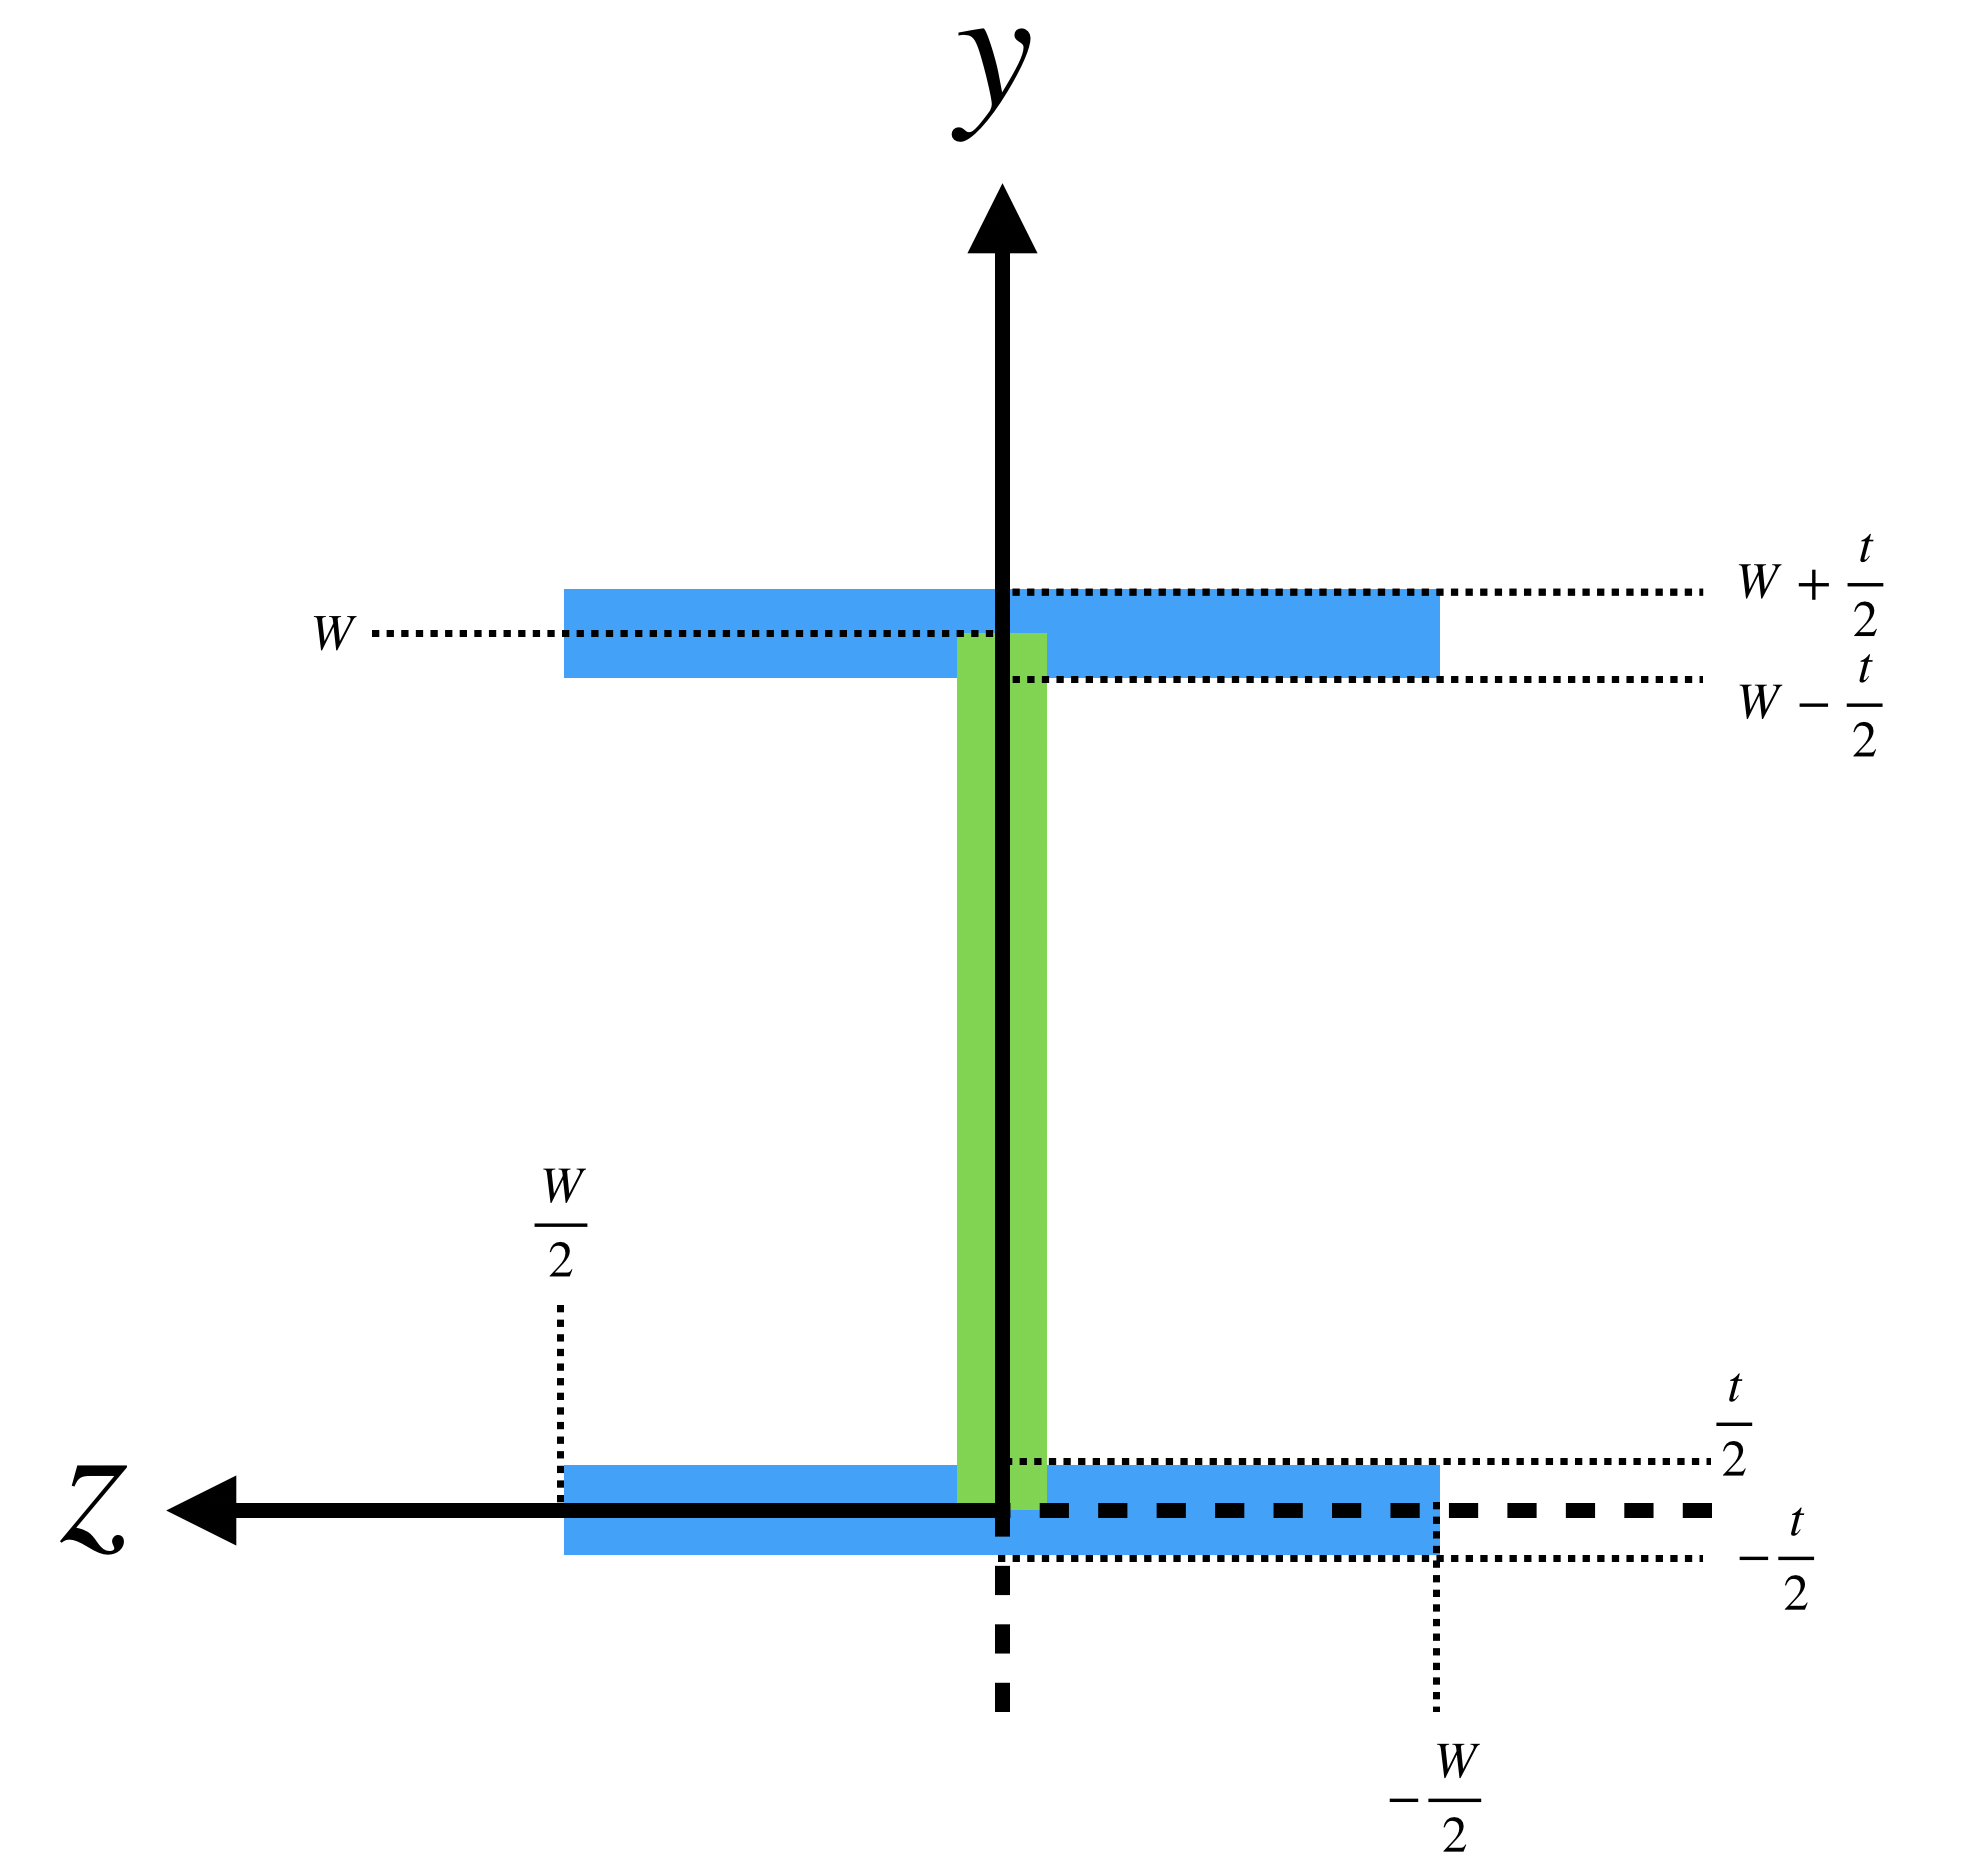
\includegraphics[width=0.7\linewidth]{images/I-beam}
	\caption{The I-beam.}
	\label{fig:i-beam}
\end{figure}
Thus
\begin{equation}
	\begin{split}
		I_y &= \iint dy \, dz \, z^2 = I_\text{bot} + I_\text{mid} + I_\text{top} \\
		&= \int_{-\frac{ t }{ 2 }}^{\frac{ t }{ 2 }} dy \int_{-\frac{ W }{ 2 }}^{\frac{ W }{ 2 }} dz \, z^2
		+ \int_{0}^{W} dy \int_{-\frac{ t }{ 2 }}^{\frac{ t }{ 2 }} dz \, z^2
		+ \int_{W - \frac{ t }{ 2 }}^{W + \frac{ t }{ 2 }} dy \int_{-\frac{ W }{ 2 }}^{\frac{ W }{ 2 }} dz \, z^2 \\
		&= t \frac{ W^3 }{ 12 } + W \frac{ t^3 }{ 12 } + t \frac{ W^3 }{ 12 } \\
		&= t \frac{ W^3 }{ 6 } + W \frac{ t^3 }{ 12 }.
	\end{split}
\end{equation}
And
\begin{equation}
	\begin{split}
		I_z &= \iint dy \, dz \, y^2 = I_\text{bot} + I_\text{mid} + I_\text{top} \\
		&= \int_{-\frac{ t }{ 2 }}^{\frac{ t }{ 2 }} dy \, y^2 \int_{-\frac{ W }{ 2 }}^{\frac{ W }{ 2 }} dz
		+ \int_{0}^{W} dy \, y^2 \int_{-\frac{ t }{ 2 }}^{\frac{ t }{ 2 }} dz
		+ \int_{W - \frac{ t }{ 2 }}^{W + \frac{ t }{ 2 }} dy \, y^2 \int_{-\frac{ W }{ 2 }}^{\frac{ W }{ 2 }} dz \\
		&= W \frac{ t^3 }{ 12 } + \frac{ W^3 }{ 3 } t + \frac{ 1 }{ 3 } \Big( 3 t W^2 + \frac{ t^3 }{ 4 } \Big) W \\
		&= \frac{ t^3 }{ 6 } W + \frac{ 4 }{ 3 } t W^3.
	\end{split}
\end{equation}

\subsection{3}
If the I-beam is simply supported at both ends at $x=0$, $x=L$, and a load $P$ is placed in the center of the beam at $x=L/2$,
\begin{enumerate}[(a)]
	\item Determine the bending moment

	      \textbf{Solution:}
	      \begin{figure}[h]
		      \centering
		      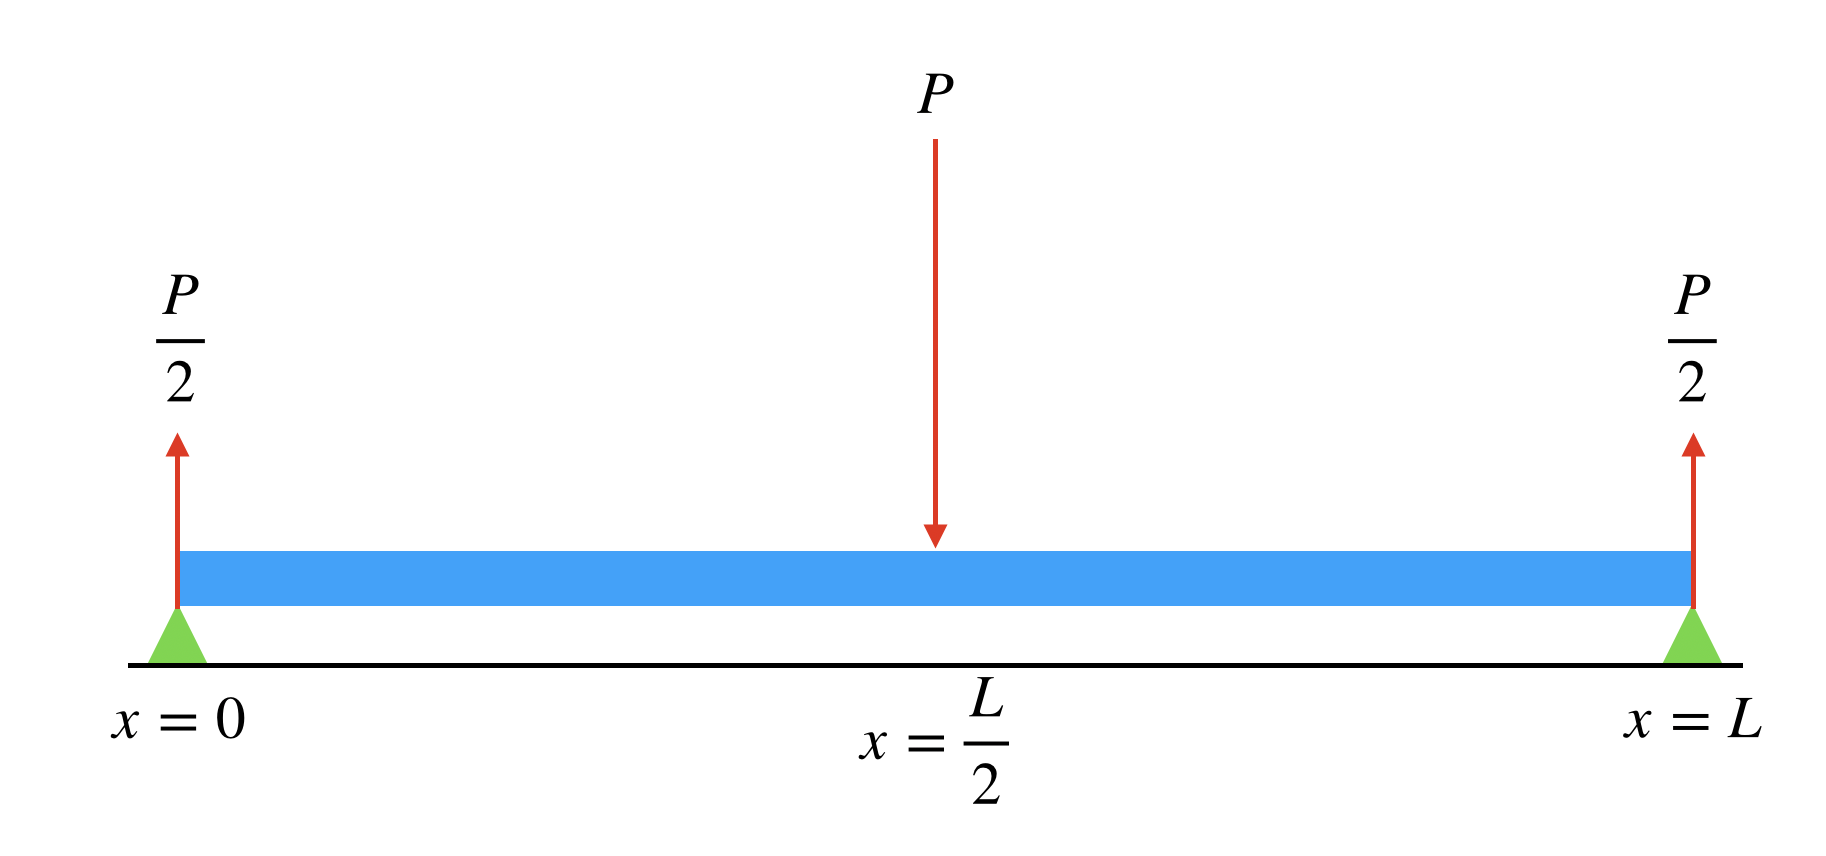
\includegraphics[width=0.6\linewidth]{images/support}
		      \caption{Schematic plot.}
		      \label{fig:support}
	      \end{figure}
	      For simple support, the heights $y(0)$, $y(L)$ are constrained to $0$.
	      The shear $\sigma_{yx}$ through the beam is assumed to be $0$.
	      There are only normal (point) stresses $\sigma_{yy}$ at both ends. (The end faces can rotate.)
	      Zero $\sigma_{yx}$ implies constant bending moment $M_z$ throughout the beam, denoted as
	      $M$ here. (This situation is known as ``pure bending".)
	      It is the same for $z$ direction loading by symmetry, so $M_y = M$.
	      Here we let $M$ be equal to the moment of the three-point bend $\dfrac{ P L }{ 4 }$.

	\item For Young's modulus $E$, what will be the curvature of the beam if the load is placed in
	      \begin{enumerate}[(b1)]
		      \item the $z$ direction,
		      \item the $y$ direction?
	      \end{enumerate}
	      (If the load is due to gravity this corresponds to rotating the beam about its long axis.)

	      \textbf{Solution:}
	      \begin{enumerate}[(b1)]
		      \item Similar to equation $(2.29)$,
		            \begin{equation}
			            \begin{split}
				            \bigg| \frac{ \partial^2 z }{ \partial  x^2} \bigg| &= \frac{ M_y }{ E I_y }\\
				            &= \frac{ 1 }{ E  \big( t \frac{ W^3 }{ 6 } + W \frac{ t^3 }{ 12 } \big)} \frac{ P L }{ 4 }.
			            \end{split}
		            \end{equation}
		      \item Based on the same reason,
		            \begin{equation}
			            \begin{split}
				            \bigg| \frac{ \partial^2 y }{ \partial x^2 } \bigg| &= \frac{ M_z }{ E I_z } \\
				            &= \frac{ 1 }{ E \big( \frac{t^3 W}{6} + \frac{4 t W^3}{3} \big)} \frac{ P L }{ 4 }.
			            \end{split}
		            \end{equation}
	      \end{enumerate}
	\item Determine the maximum stress on the beam for the two orientations.

	      \textbf{Solution:}

	      Similar to equation $(2.16)$, for force pointing toward $y$ direction, we will have
	      \begin{align}
		      | \sigma_y | & = E \frac{ y }{ R_y }, \\
		      | \sigma_z | & = E \frac{ z }{ R_z },
	      \end{align}
	      where
	      \begin{align}
		      R_y^{-1} & = \bigg| \frac{ \partial^2 y }{ \partial x^2 } \bigg|, \\
		      R_z^{-1} & = \bigg| \frac{ \partial^2 z }{ \partial  x^2} \bigg|.
	      \end{align}
	      So
	      \begin{align}
		      | \sigma_y | & = E y \bigg| \frac{ \partial^2 y }{ \partial x^2 } \bigg| = y \frac{ 1 }{ \big( \frac{t^3 W}{6} + \frac{4 t W^3}{3} \big)} \frac{ P L }{ 4 },        \\
		      | \sigma_z | & = E z \bigg| \frac{ \partial^2 z }{ \partial  x^2} \bigg| = z \frac{ 1 }{ \big( t \frac{ W^3 }{ 6 } + W \frac{ t^3 }{ 12 } \big)} \frac{ P L }{ 4 }.
	      \end{align}
	      The maxima $|\sigma_y|$ and $|\sigma_z|$ reach when $|y|$ and $|z|$ are at their maxima.
	      Since the neutral axis must be at the midpoint of the beam,
	      $-\frac{ t }{ 2 } \le y \le \frac{ t }{ 2 }$, $-\frac{ W }{ 2 } \le z \le \frac{ W }{ 2 }$. Thus,
	      \begin{align}
		      | \sigma_y |_\text{max} & = \frac{ t }{ 2 } \frac{ 1 }{ \big( \frac{t^3 W}{6} + \frac{4 t W^3}{3} \big)} \frac{ P L }{ 4 },        \\
		      | \sigma_z |_\text{max} & = \frac{ W }{ 2 } \frac{ 1 }{ \big( t \frac{ W^3 }{ 6 } + W \frac{ t^3 }{ 12 } \big)} \frac{ P L }{ 4 }.
	      \end{align}
\end{enumerate}

% \bibliographystyle{unsrt}
% \bibliography{ref}

% --------------------------------------------------------------
%     You don't have to mess with anything below this line.
% --------------------------------------------------------------

\end{document}